\newpage


\section{Przegląd literatury -- SZKIELET POZIOMU 2}
\label{sec:literature}

1. Akapit wstępny o różnych podejściach do partycjonowania.
O tym, że wyróżniamy dwa podstawowe podejścia:

\begin{itemize}
    \item {\cite{metis} - duzo o roznych metodach - mozna uwzglednic}
    \item{siatka jest dzielona od razu na docelową liczbę partycji (podejście, które stosuję) - multilevel partitioning}
    \item{Siatka jest dzielona na dwie części, następnie rekursywnie dzielimy każdą z nich aż do otrzymania oczekiwanej
    liczby partycji}
\end{itemize}

2. Akapit o rekursywnym dzieleniu siatek.
\begin{itemize}
    \item {że przykładowo jest algorytm\cite{recursive}, zakładający żę dzielimy siatkę na liczbę obszarów,
        która jest równa potędze liczby dwa, algorytm potrafi także dzielić siatkę wedle możliwości obliczeniowych
        poszczególnych rdzeni procesora. Dzielenie na liczbę obszarów równą potędze liczby jest poważnym ograniczeniem
        wykluczającym zastosowanie tego algorytmu.}
    \item{inne przykłady takich algorytmów}
    \item {Akapit na temat tego że są to metody prostsze w implementacji, jednak nie sprawdzają się tak dobrze w kontekście bardziej
    skomplikowanych problemów głównie ze względu na to, że mają zachłanną naturę.
    Ponadto wykorzystanie takich algorytmów w kontekście niepodzielnych obszarów nie zdaje egzaminu,
        ze względu na ich specyfikę. Podejście do partycjonowania zakładające dzielenie grafu na coraz mniejsze
        części sprawia, że nie jesteśmy w stanie uwzględniać części niepodzielnych, lub rozwiązanie tego problemu byłoby skomplikowane.
        Przykład - dzielimy siatkę na 4 części. Można sobie wyobrazić sytuację, kiedy obszar niepodzielny zajmuje 50\% całej siatki.
        Po pierwszej turze rekursywnego algorytmu mamy dwie partycje, każda zajmująca 50\% powierzchni. Chcielibyśmy podzielić
        każdą z nich na dwie części, natomiast nie jesteśmy w stanie tego zrobić ponieważ jedna z nich jest w całości obszarem
        niepodzielnym.}
    \item {Po wymienieniu powyższych wad wstęp do kolejnego akapitu, który mówi o tym, że w kontekście obszarów niepodzielnych
    lepiej sprawdzają się algorytmy typu multilevel partitioning.}
\end{itemize}

\newpage
3. Akapit o dzieleniu siatek na docelową liczbę części
\begin{itemize}
    \item {Że są to metody często szybsze od metody rekursywnych\cite{KARYPIS199896}}
\end{itemize}

\begin{wrapfigure}{r}{0.6\textwidth}
    \vspace{-4mm}
    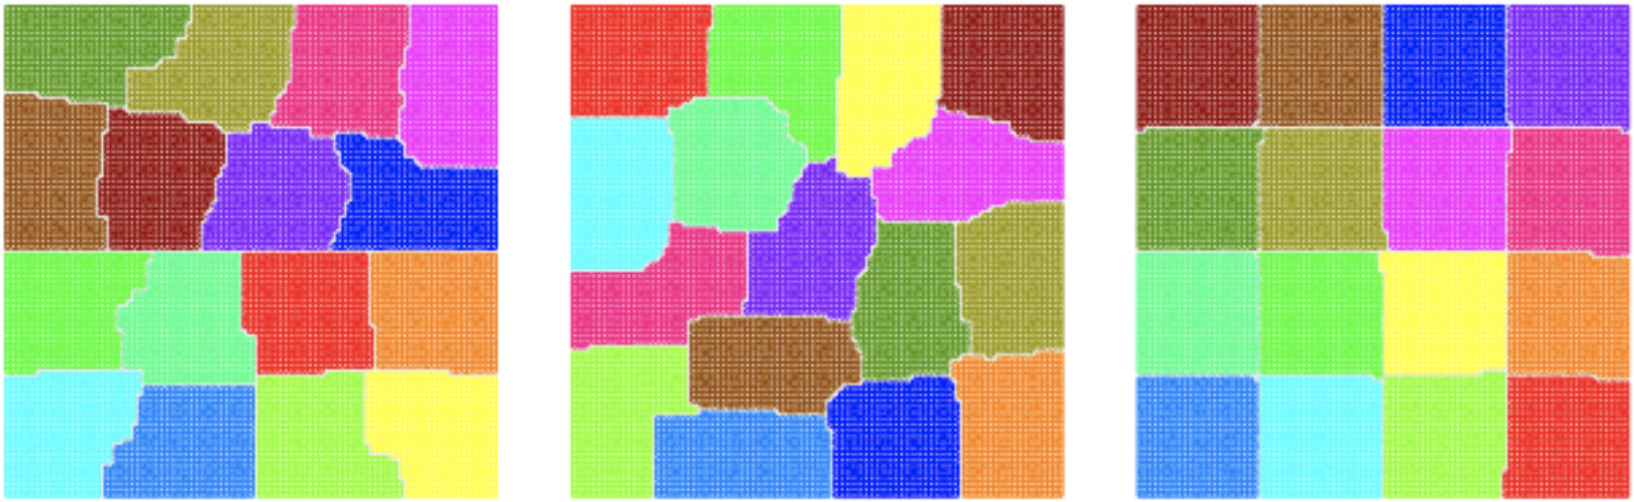
\includegraphics[width=\linewidth]{images/libraries-comparision}
    \caption{Partycjonowanie siatki 100x100 na 16 obszarów. Od lewej - pmetis\cite{metis} uzyskuje edge-cut wynoszący
    688, następnie Jostle\cite{jostle} z wynikiem 695 oraz Party\cite{1364754} z wynikiem 615.}
    \label{fig:test2}
\end{wrapfigure}

\lipsum

